%========================= CAPITULO 3 ==============================

\chapter{Falhas e Análise de Requisitos} %\label{cap_exemplos}
%\thispagestyle{empty}
\section{Falhas Apontadas e Obervadas}
Com aplicação do questionário e o com o período de permanecia do teleatendimento da Polícia Militar de Dourados, ficou evidente algumas falhas técnicas e mesmo humanas neste teleatendimento.

\subsection{Aplicação do Questionário}
O questionário foi aplicado não somente com objetivo de apontar falhas, mas também de saber quais as opiniões dos policiais do teleatendimento tem sobre os atuais equipamentos utilizados por eles, e ainda saber sobre as possíveis melhorias advindas das funcionalidades da ferramenta Asterisk.

Logo todos consideram que o seu trabalho é essencial para à sociedade e que o
primeiro contado do cidadão é por intermédio deste teleatendimento, porém 85\% dos teleatendentes, não consideram que seu  local de trabalho tem o necessário para um atendimento de excelência a sociedade, bem como, não tem o equipamento ideal para prestar esse serviço.

E na questão \textbf{``Você sabe precisar quantas ligações o sistema de telefonia emergencial atende diariamente, e quantas dessas ligação, realmente são ocorrências, e quantas são trotes, pedidos de informação? Se sim informe a quantidade.''}, 57\% responderam que sim, porém com valores desencontrados a exemplo o número de ocorrências de um foi 30 já outro foi 70 e assim também foi para os outros questionamentos, percebe que não há como contabilizar a quantidade de atendimentos diários.

No questionário que tece questões sobre aprimoramentos do teleatendimento através das funcionalidades da ferramenta Asterisk, a questão \textbf{``Você acredita que um sistema de telefonia onde possa gravar e identificar a ligações para este teleatendimento, agregaria vantagens?''}, somente um respondeu que não, pois segundo ele, “A população e hipócrita e mal educada usaria isto em desfavor da PM”, percebe que não há como gravar as chamadas, e que por mais que isso seja uma melhoria, na visão deste pode ser maleficio.

Todos os atendentes acreditam que um sistema que possam criar uma fila de espera e onde esta prioriza o atendente que esta mais tempo sem atender, seja o escalado para a próxima chamada, e todos também creem que um sistema de captura e transferência de chamadas é uma melhoria no teleatendimento, bem como, um sistema de teleconferência.

\subsection{Falhas Humanas}
Apesar destas falhas não serem objetos de estudo deste trabalho, não deixam de ser um fator preocupante para a eficiência do teleatendimento. E ainda estas falhas acabam relacionando-se indiretamente ou diretamente com algumas falhas técnicas que serão apontadas.

Uma falha verificada foi com relação aos PA (\textit{Pontos de Atendimentos}), ou seja, quando um policial por algum motivo necessita se ausentar de sua cabine de atendimento e porventura acaba esquecendo de desabilitar o seu PA, isso gera um transtorno para o solicitante pois, a ligação deste solicitante acaba caindo neste PA com o atendente ausente, só que para o solicitante que esta em uma situação urgência, emergência esta sendo gerado tom de chamada, e como consequência ele não é atendido.

Outra falha que coexiste com a anterior, é o fato que o outro atendente tem que se levantar de sua cabine, seja para atender a chamada de seu colega de trabalho ou mesmo derrubá-la, ou seja, desabilitar o PA do colega enquanto ocorre uma chamada de um solicitante ou ignorá-la.

E os policiais além de terem que atender as chamadas, ainda tem que ser despachadores, ou seja, despachar as ocorrências com as viaturas, e nesse momento outra chamada é recebida no PA deste atendente e o mesmo fica impossibilitado de atender esta chamada devido a estar passando as informações da solicitação anterior para a viatura, logo ele ignora ou derruba a chamada.

A ferramenta Asterisk tem funcionalidades técnicas como DAC (\textit{Distribuição Automática de Chamadas}) ou captura de chamadas para amenizar ou mesmo cessar as falhas humanas apresentadas.

A funcionalidade conhecida como DAC ou filas de atendimento, é a maneira que o Asterisk enfileira as chamadas de entrada do servidor, para que posteriormente seja encaminhadas para os agentes de atendimento \cite{flavioeduardoandredade2005}.

Esta funcionalidade geralmente é empregada em \textit{call centers}. E existem dois tipos, os ativos que originam chamadas para o cliente externo oferecendo planos, promoções, etc, e os receptivos, pois trata apenas de chamadas de entrada no sistema, logo o teleatendimento da Polícia Militar se encaixa nesta segunda abordagem. A DAC trás inúmeras vantagens para o teleatendimento, pois organiza as ligações de entrada, e ainda pode-se configurar os atendente para logar-se no servidor PABX, e caso se necessário pode definir um tempo em segundos de inatividade para os atendentes e o próprio servidor coloca este atendente como impossibilitado de atender uma chamada \cite{alexandrekeller2014}.

Captura de chamadas permite que o atendente puxe para seu ramal uma chamada de outro atendente no qual seu ponto de atendimento esta tocando, e pode ser em grupo onde os atendentes pertencem ao mesmo grupo, porém, apenas funciona para canais de comunicação com o mesmo protocolo, ou seja, um canal de comunicação SIP, só pode capturar chamadas de canais de comunicação definidos com SIP. E ainda pode ser direta onde o atendente pode capturar a chamada diretamente discando o número do ramal que se deseja capturar. Esta funcionalidade evita que o atendente tenha que se levantar ou deslocar de sua cabine de atendimento para atender uma PA de outro atendente que esteja tocando \cite{alexandrekeller2014}. 

\subsection{Falhas Técnicas}
As falhas humanas apresentadas, também podem ser consideradas falhas técnicas, pois, no atual momento deste teleatendimento não há nenhuma ferramenta para inibir ou mesmo cessar as falhas identificadas como humanas, porém como demonstrado com as funcionalidades da ferramenta Asterisk podemos saná-las.

A falta de um controle de agentes é uma falha técnica, pois, não há nenhum controle de quando o atendentes ficaram disponíveis para o atendimento das chamadas ou mesmo indisponíveis.

Não existe controle das ligações, ou seja, quantos atendimentos diários foram realizados, quantos desses atendimentos eram realmente ocorrências, quantos eram trotes, pedidos de informação, não há possibilidade do levantamento de estatísticas das ligações recebidas.

Logo não há gravação do áudio das chamadas, isto gera um transtorno tanto para os atendentes como para os cidadãos, pois, caso ocorra uma reclamação contra um atendente, não há como verificar como procedeu o atendimento. E ainda não há uma identificação desta chamadas, mas comumente conhecido como bina, que nada mais é que um serviço telefônico que permite ao assinante chamado identificar o número do terminal originador da chamada.

Outro fator preocupante é a falta da possibilidade de transferência de chamadas, pois, foi verificado que é comum um cidadão retornar a ligação, seja para complementar a solicitação, passar ou repassar algumas informações relevantes para o atendimento, ou mesmo para reportar alguma reclamação, e fica evidente que geralmente o solicitante quer e precisa falar com quem o atendeu anteriormente, e quando este liga novamente acaba sendo atendido por outro. Isso torna-se oneroso pois coleta as informações e repassa posteriormente, ou cede seu PA para o policial anterior complementar as informações, ficando este ocioso.

No teleatendimento, não há uma organização dos ramais, ou seja, não há uma estratégia de atendimento, isto ocasiona uma deficiência com relação ao recebimento das chamadas nos ramais, pois, o primeiro ramal sempre recebera mais ligações do os outros ramais, pelo fato que não há inteligencia no sistema de telefonia, logo se o primeiro ramal estiver desocupado, uma ligação cairá neste ramal, somente quando este estiver ocupado passará para o segundo ramal, isso segue sucessivamente.

Não tem uma padronização no atendimento, ou seja, não há uma mensagem inicial no primeiro contato como uma mensagem de boas vindas para identificar de qual órgão de segurança pública se trata, isto se faz necessário, pois, alguns cidadãos confundem os números emergenciais dos órgãos de segurança públicas.

Os equipamentos utilizados no teleatendimento da Polícia Militar são de uso continuo, e já tem longa data de utilização, e muitos estão apresentando defeitos e avarias, e fica evidente a falta de manutenção ou mesmo a troca devido seu valor elevado.

Assim como nas falhas humanas a ferramenta Asterisk tem funcionalidades como a própria DAC, gravação de chamadas, transferência de chamadas ou teleconferência e bilhetagem para amenizar ou cessar as falhas técnicas deste teleatendimento.

A DAC além de auxiliar nas falhas humanas apresentadas anteriormente, pode auxiliar no controle dos atendentes, pois, estes terão que autenticar-se no sistema para poderem atenderem as chamadas, e com auxilio de outra funcionalidade que é a bilhetagem podemos ter todas informações de autenticação dos usuários, bem como, controle de todas as informações das chamadas, identificação da chamada, tempo médio de espera, tempo médio de atendimento, quantidade chamadas abandonadas, ou seja, aquelas que o cidadão desistiu, e ainda criar estrategias de atendimento para os atendentes, ou seja, a chamada vai cair para o atendente que esta mais tempo sem atender uma chamada, aquele que não concretiza um atendimento, aleatoriamente entre outras \cite{books/daglib/0018909}.

A DAC ainda permite uma padronização do atendimento, pois pode empregar uma URA, com uma mensagem identificando o órgão de segurança pública, e caso tenha pelo menos um atendente disponível transfere a chamada para ele, caso tenha mais de um, utiliza uma das estrategias de atendimento mencionados no paragráfo anterior, e não havendo nenhum, cai direto na fila de atendimento, e pode informar com uma mensagem automatica a posição a qual se encontra na fila, ou seja, quantos estão na sua frente aguardando o atendimento e ou ainda colocar uma musica em espera \cite{flavioeduardoandredade2005}.

Bilhetagem é o armazenamento de todas as informações de todas as chamadas executadas ou recebidas, podem ser simplesmente arquivos de texto simples ou ainda serem armazenados em banco de dados externos como MySQL ou Postgresql através de ODBC (\textit{Open Database Connectivity})\footnote{Padrão aberto de conectividade com praticamente qualquer banco de dados disponível}. Porém bilhetagem não é tarifação, ou seja, cobrança de custos das ligações \cite{alexandrekeller2014}.

A gravação da chamadas podem ser a nível de atendente ou não própria configuração da fila, e ainda pode ser implementada de duas formas, sendo por meio de aplicação onde toda chamada e gravada e não existe a possibilidade de interrompê-la, ou sobre demanda que só inicia a gravação por intermédio da digitação de um comando digitado. Saliente informar que a gravação esta entre as funcionalidades que mais consomem recursos, pois dependem da velocidade do disco utilizado \cite{alexandrekeller2014}.

Outra vantagem da ferramenta Asterisk e com relação ao equipamento, pois pode ser empregado ATA's, telefones analógicos comuns através de uma placa FXS instalada no servidor PABX ou ainda softfones instaladas no próprios computadores dos atendentes e nesta ultima opção necessita apenas de um headfone para comunicação, porém este ainda tem um preço bem mais atrativo que os headsets, logo sua manutenção, reparo ou mesmo troca terá um custo mais baixo.

\section{Requisitos Necessários}
A ferramenta Asterisk faz o elo de ligação entre a PSTN e o VoIP, ou seja, é considerada um servidor PABX híbrido. Mas para essa finalidade ela necessita de requisitos para sua implantação, logo, serão abordados os requisitos necessários para aplicar a ferramenta Asterisk no cenário escolhido, que é o teleatendimento emergencial da Polícia Militar de Dourados.

\subsection{Telefônia}
No teleatendimento existem quatro ramais analógicos administrados pela operadora de telefonia, que chegam no quadro de distribuição através de cabo FE\footnote{Fio telefônico para instalações aéreas} e posteriormente e distribuídos até os PA dos atendentes.

Para a ferramenta fazer a integração da telefonia convencional com o VoIP, foi adquirida uma placa TDM410P 4 portas FXO (\textit{recebe tom de discagem}) para conexão com os atuais ramais analógicos do teleatendimento, porém, a ferramenta disponibilizará internamente os ramais por meio da LAN, ou seja, por intermédio da VoIP, logo, este teleatendimento contará com todas as funcionalidades da ferramenta Asterisk. A placa é ilustrada na figura \ref{Figura16}.

\begin{figure}[h]
	\centering
	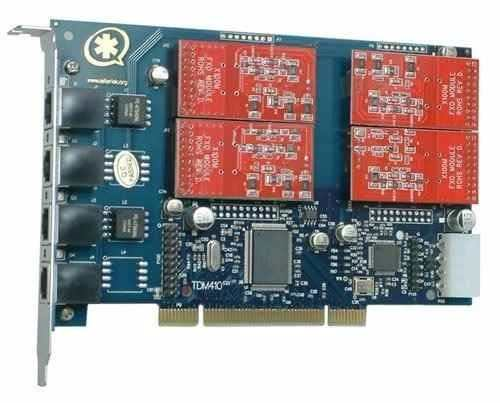
\includegraphics[width=8cm]{imagens/tdm410p.jpg}
	\caption{Placa TDM410P 4 portas.}
    \label{Figura16}
\end{figure}

\subsection{Rede de Computadores}
A LAN (\textit{Local Area Network}) ou rede de computadores local deve receber uma atenção especial desde o momento do projeto para a implementação de serviços com base VoIP, pois, a qualidade do áudio trafegado é afetado por fatores diretamente ligados à rede como o tamanho da banda, latência e jitter \cite{andersonramires2005}.

A rede de computadores do teleatendimento é composta por cabos de par trançado de categoria 5, e é interligada através de switch central com barramento 10/100 de 24 portas, e nas estações de trabalho (\textit{computadores}) o barramento das placas ethernet (\textit{placa de rede}) é de 10/100. A ilsutração do switch interligando as estações de trabalho pode ser vista através da figura \ref{Figura17}

\begin{figure}[h]
	\centering
	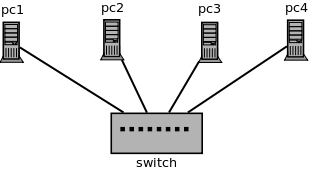
\includegraphics[width=8cm]{imagens/switch.png}
	\caption{Conexão entre o switch e as estações de trabalho.}
    \label{Figura17}
\end{figure}

\subsection{Hardware}
O teleatendimento não possui um computador exclusivo para a ferramenta Asterisk, então foi adquirido um computador com configurações razoáveis porém compatível com o cenário pretendido. O hardware foi escolhido acima do dimensionamento pretendido para o cenário, pois devido ao teleatendimento possuir somente quatro ramais analógicos, logo poderá ter somente quatro chamadas simultâneas. \citeonline{alexandrekeller2014} expõe que a quantidade de chamadas simultaneas e se ira gravar as chamadas e velocidade do disco são fatores para dimensionamento correto do hardware. 

\begin{figure}[h]
	\centering
	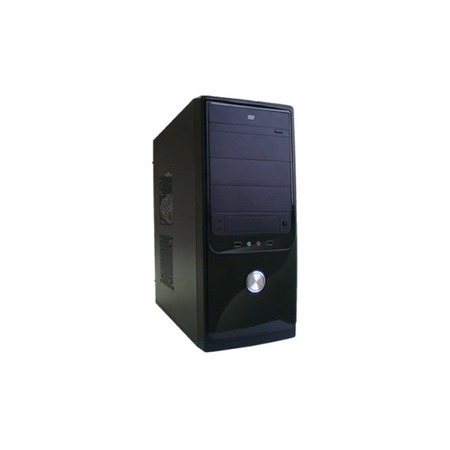
\includegraphics[width=6cm]{imagens/gabinete.jpg}
	\caption{Computador para o servidor PABX.}
    \label{Figura18}
\end{figure}

\subsection{Software}
O sistema operacional\footnote{Um sistema operacional é um conjunto de programas básicos e utilitários que fazem seu computador funcionar} escolhido para a instalação da ferramenta Asterisk foi a ultima versão estável do GNU/Linux Debian. O Debian é um sistema operacional de distribuição não comercial e livre que usa o kernel Linux. A versão oito do Debian com codinome Jessie é sua ultima versão estável, os desenvolvedores do Debian sempre homanegencia suas versões com nomes dos personagens do filme Toy Story\footnote{Toy Story é um filme estadunidense de aventura e comédia de 1995. É conhecido por ser o primeiro longa-metragem dos estúdios Pixar e também o primeiro da história totalmente feito por computação} \cite{valessiosoaresbrito2015}.

Além de ser um sistema operacional de distribuição livre, o Debian é uma distribuição de alta qualidade, estável e escalável, que podem ser facilmente configurado para servir em vários papéis, desde firewalls dedicadas a ambientes de estações de trabalho científico e até servidores de rede de elevada gama, e é especialmente popular entre utilizadores mais avançados devido à sua excelência técnica e ao seu profundo compromisso com as necessidades e expectativas da comunidade Linux \cite{valessiosoaresbrito2015}.

